\documentclass[12pt]{article}
\usepackage{ctex}
\usepackage[left=1.81cm, right=1.81cm, top=1.81cm, bottom=1.81cm]{geometry}
\usepackage{amsmath, amsfonts, amssymb} % 数学公式、符号
\usepackage{graphicx}   % 图片
\usepackage{url}        % 超链接
\usepackage{bm}         % 加粗方程字体
\usepackage{multirow}
\usepackage{array}
\usepackage{graphicx}
\usepackage{caption}
\usepackage{booktabs}
\usepackage[T1]{fontenc}
\usepackage{fancybox}
\usepackage{wrapfig}
\usepackage{multicol}
\usepackage{enumerate}
\renewcommand{\thesection}{\zhnum{section}}
\renewcommand{\thesubsection}{\arabic{subsection}}
\renewcommand{\thesubsubsection}{(\arabic{subsubsection})}
\newcommand*{\expname}{\large{RLC电路的稳态}}
\newcommand*{\name}{姓名}
\newcommand*{\nianji}{年级}
\newcommand*{\stdnum}{学号}
\newcommand*{\expdate}{日期}
\setlength{\parindent}{4em}
\begin{document}
\begin{center}
	\kaishu\pmb{\Huge{武\ 汉\ 大\ 学\ 物\ 理\ 科\ 学\ 与\ 技\ 术\ 学\ 院}}\\
	\kaishu\Huge{\pmb{物\ 理\ 实\ 验\ 报\ 告}}
\end{center}
\renewcommand\arraystretch{1.5}
\begin{tabular*}{\linewidth}{|m{1.81cm}<{\raggedright}|m{2.51cm}<{\raggedright}|m{1.31cm}<{\raggedright}|m{1.61cm}<{\raggedright}|m{1.31cm}<{\raggedright}|m{3.3cm}<{\raggedright}|m{1.31cm}<{\raggedright}|m{1.31cm}<{\raggedright}|}
	\multicolumn{3}{r}{\large \heiti {物理科学与技术学院}}&\multicolumn{2}{r}{\large \heiti {物理学专业}}&\multicolumn{3}{r}{\large\heiti {\expdate}}\\
	\hline
	实验名称&\multicolumn{7}{l|}{\expname }\\
	\hline
	姓\ \ \  \ \  \ 名&\raggedright\name  &年\ \  \ 级 &\nianji &学\ \ \ 号& \stdnum &成\ \  绩 & \ \\
	\hline
	\multicolumn{8}{|l|}{
		\begin{minipage}[h]{0.928\columnwidth}
			\renewcommand\arraystretch{1}
			\begin{tabular}{m{9cm}p{5cm}}
				实验报告内容: &                      \\
				一、实验目的 &               五、数据表格 \\
				二、主要实验仪器 &          六、数据处理及结果表达 \\
				三、实验原理 &            七、实验结果分析 \\
				四、实验内容与步骤 &           八、习题 \\
				\end{tabular}  
		\end{minipage}
	}\\
	\hline
	\multicolumn{8}{|c|}{
		\begin{minipage}[h]{0.928\columnwidth}
			\raggedright
			{\fancypage{\fbox}{}
\section{实验目的}
\begin{enumerate}
    \item 目的1
    \item 目的2
    \item 目的3
    \item 目的4
\end{enumerate}

\section{实验仪器}
~\\
~\\
~\\












}
	\end{minipage}
	}\\
	\hline
\end{tabular*}	
\renewcommand\arraystretch{1}
\fancypage{\fbox}{}
\subsubsection{幅频特性}
根据上述$U_R,U_C$的表达式,当$\omega \rightarrow 0$时,$U_R\rightarrow 0,U_C\rightarrow U$;$U_R$随着$\omega$增大逐渐增大,$U_C$反之;当$\omega \rightarrow \infty$时,$U_R\rightarrow U,U_C\rightarrow 0$。
\subsubsection{相频特性}
当$\omega$很低时,$\varphi_R→+\pi/2$;当$\omega$很高时,$\varphi_R→0$,且$\varphi_C=|\varphi_R|-\pi/2$
\subsubsection{等幅频率}
\begin{wrapfigure}[6]{r}{0.3\textwidth} %比如{r}{0.5\textwidth}
	\centering
	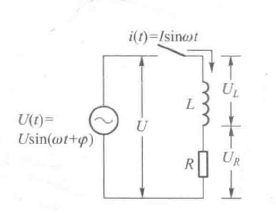
\includegraphics[height=3cm,width=5cm]{figure/2.png}
    \caption*{RL串联电路}
\end{wrapfigure}
当$R=1/(\omega C)$时,$U_R=U_C$,此时的频率为等幅频率,也叫截止频率
\subsection{RL电路的幅频特性}
RL的阻抗为$\tilde{Z}=R+j\omega L$,其模为$Z=|\tilde{Z}|=\sqrt{R^2+(\omega L)^2}$其他同RC电路
\subsection{RLC串联电路}
\begin{wrapfigure}[6]{r}{0.3\textwidth} %比如{r}{0.5\textwidth}
	\centering
	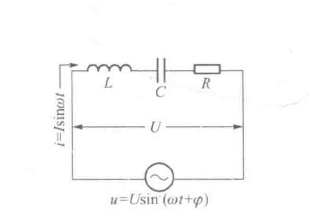
\includegraphics[height=3cm,width=5cm]{figure/3.png}
    \caption*{RLC串联电路}
\end{wrapfigure}
该电路的总阻抗为$\tilde{Z}=R+j\left(\omega L-\dfrac{1}{\omega C}\right)$

幅角:$\varphi=\arctan \dfrac{\omega L-\frac 1 {\omega C}}{R}$

R上的电压为$U_R=\dfrac{U}{Z}R $
\subsubsection{谐振频率}
当$\omega L-\dfrac{1}{\omega C}=0$时,$\varphi=0$,并且$U_R=U$为极大值,此时的频率记为谐振频率$f_0=\dfrac{1}{2\pi\sqrt{LC}}$
\subsubsection{相频特性}
$\omega <\omega _0 $时,此时电路呈电容性;$\omega >\omega _0 $时,此时电路呈电感性;$\omega =\omega _0 $时,此时电路呈电阻性。
\section{实验内容与步骤}
\subsection{测量并绘制RC串联电路的幅频、相频曲线}
\begin{enumerate}[(1)]
    \item 连接电路,接通各个仪器电源进行预热
    \item 调节信号源的$f=500Hz,U=3.0V_{RMS}=8.5Vpp$
    \item 依次从电压表上测出R,C上的电压U,U,.从示波器的李萨如图形上读出x轴与  图形相交的水平距离$2x_0$和图形在x轴上的投影$2X$
    \item 依次测出表格中其余$f$值条件下的$U_R,U_C$,和$\varphi$值.
\end{enumerate}
\subsection{测量并绘制RL串联电路的幅频、相频曲线}
与上一步内容相似,将C替换为L
\subsection{测量并绘制RLC串联电路的相频曲线}
其测量电路与以上内容相仿,只是将串联LC代替原来的C即可
\begin{enumerate}[(1)]
    \item 用李萨如图形找出谐振频率
    \item 测出f=350,600,700,780,900,1500Hz条件下的$\varphi$值
\end{enumerate}
\section{数据表格}
\begin{table}[h]
    \centering
    \caption*{RC幅频,相频曲线}
    \begin{tabular}[\linewidth]{|m{2cm}|m{2cm}|m{2cm}|m{2cm}|m{2cm}|m{2cm}|m{2cm}|}
        \hline
        \multicolumn{7}{|c|}{$U=3.0V_{RMS}=8.5Vpp$  $R=200\Omega $  $C=0.47\mu F$}\\
        \hline
        $f/Hz$ & 500 & 1200 & 1700 & 2000 & 3000 & 7000 \\
        \hline
        $U_R/V$ & & & & & & \\
        \hline
        $U_C/V$ & & & & & & \\
        \hline
        $2x_0/cm$ & & & & & & \\
        \hline
        $2X/cm$ & & & & & & \\
        \hline
        $\varphi/(^{\circ} )$ & & & & & & \\
        \hline
    \end{tabular}
    \caption*{RL幅频,相频曲线}
    \begin{tabular}[\linewidth]{|m{2cm}|m{2cm}|m{2cm}|m{2cm}|m{2cm}|m{2cm}|m{2cm}|}
        \hline
        \multicolumn{7}{|c|}{$U=3.0V_{RMS}=8.5Vpp$  $R=1000\Omega $  $L=0.1H$}\\
        \hline
        $f/Hz$ & 500 & 1200 & 1700 & 2000 & 3000 & 7000 \\
        \hline
        $U_R/V$ & & & & & & \\
        \hline
        $U_L/V$ & & & & & & \\
        \hline
        $2x_0/cm$ & & & & & & \\
        \hline
        $2X/cm$ & & & & & & \\
        \hline
        $\varphi/(^{\circ} )$ & & & & & & \\
        \hline
    \end{tabular}
\end{table}
 
\fancypage{\fbox}{}
在这里写第四页内容\\
\begin{table}[b]
	
	\begin{tabular}
		{p{1.2cm}|p{6cm}p{6.6cm}r}
		\hline
		 & & &  \\
		\centering\textbf{\songti  \zihao{-4}教} &                      &                      &                      \\
		\centering\textbf{\songti  \zihao{-4}师} &                      &                      &                      \\
		\centering\textbf{\songti  \zihao{-4}评} &                      &                      &                      \\
		\centering\textbf{\songti  \zihao{-4}语} &  
		&                      &                       \\                                       & &\songti \zihao{5}指导教师:&\songti \zihao{5} \quad 年 \quad 月 \quad 日 \\
	\end{tabular}  
\end{table}














%%%致谢
\end{document}
